
\chapter{Firm model}
Our treatment of the urban surplus which is central to this thesis, is illustrated in Figure~\ref{fig:Agglomeration-surplus}. In the lower left, we illustrate a single firm with decreasing returns to scale operating at its optimal scale, $n$. The thick diagonal line represents the effect of increasing the number of firms operating at the optimal scale. It is the constant returns (CRS) line. If congestion effects from bringing a large number of firms together were dominant, a city would exhibit decreasing returns to  scale,  $N$, and agglomeration would not occur. Research indicates that cities exhibit increasing returns to scale, illustrated by the upper line, which shows the city generating an increasing surplus as it grows, which is the increasing returns to scale case. The curvature of the line is determined by a function of the form $N^\gamma$, which we include in the production function for urban firms. 

In this section we are describing how we embed a model of diminishing returns to scale firms within an increasing returns to scale economy. 

We assume there are many firms operating at their optimal scale in both the rural and urban sector, but the production function of the urban firm is augmented by the term $N^\gamma$. 

NOTE ON EXPONENTS

\begin{figure}[htb]
    \centering

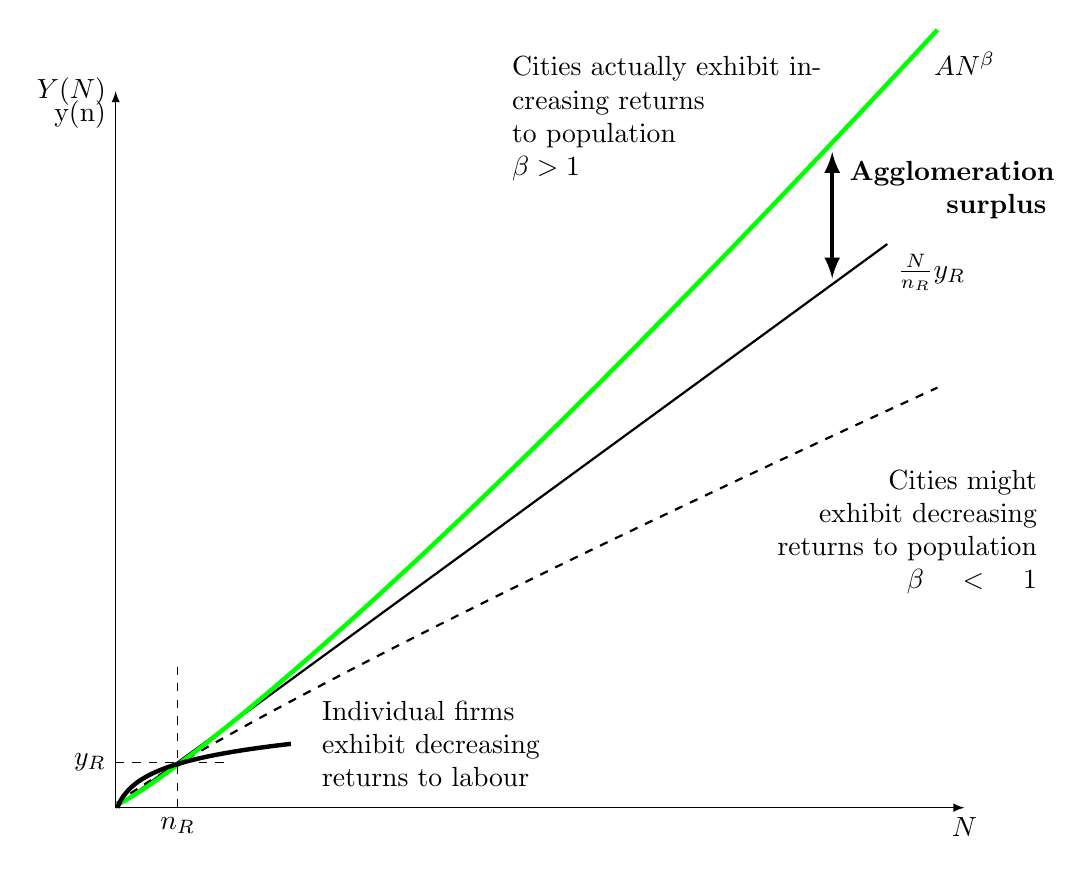
\begin{tikzpicture}[scale=.7, my plot/.style={thick, smooth, samples=100, domain=0.1:2.2},
plot2/.style={thick, smooth, samples=100, domain=0.1:14.99},
                    my grid/.style={dashed,opacity=0.5, every node/.style={black,opacity=1}},
                    my axis/.style={latex-latex}]
 
 \draw[my axis] (0,13)node[left] {$Y(N)$} --(0,0)-- (15.4, 0) node[below] {$N$}; 
%creates the axis 
 \node at (0,13)[below left]{y(n)};
 
\coordinate (origin) at (0,0);
\def\x{0.45}
\def\y{2.1}
\def\b {$15/(2*ln(\y)+.05)$};
%\def\p{0.55} % define the x, y and p )(midpointvalues
%\draw[my plot] (0,0) plot (\x,{ln(\x)});  %Draws curve
%\draw[my plot] (0,0) plot ({\x-.08},{2.3+ln(\x)}); 
\coordinate (Uy) at (\y,{2*ln(\y)+.05});

% THREE SCALE POSSIBILITIES
\draw [thick, ](0,0)--(14, 10.22583)node[below right]{$\frac{N}{n_R}y_R$};   %diagonal line CRS
\draw[plot2, dashed] (0,0) plot ({\x-.08},{(\x)^0.9/1.5 }); %DRS
\draw[plot2, ultra thick, green] (0,0) plot ({\x-.08},{(\x/1.5)^1.15});%
\node at (15.4, 13.5){$AN^\beta$};

%  TEXT
\node at (13.8,12.5) [left, text width=4.5cm]{Cities actually exhibit increasing returns\\ to population\\ $\beta>1$};%IRS
\node at (13.5,5)[text width=4.5cm, align=right] {Cities might\\ exhibit decreasing \\returns to population \\ $\beta<1$};% DRS

% ARROW
\draw[latex-latex, ultra thick] (13, 11.9)--(13, 9.6);
\node at (15.1, 11.2)[ text width=2.5cm, align=right]{\textbf{Agglomeration\\ surplus}};
%\draw[latex-latex] (13, 8.4)--(13, 9.5)node [below right, text width=1.5cm]{\textbf{$\pi$}};

\begin{scope}[ yscale=.75,xscale=1.5]% shift={(1.9,0)} ,
	\coordinate (Uy) at (\y, {2.3+ln(\y)});
  \draw[my plot,ultra thick] (0,0) plot ({\x-.08},{1.15+ln(\x)/2})node[right=.25cm, text width=3.9cm]{Individual firms\\ exhibit decreasing\\ returns to labour}; % production function for generic ferm
	\draw[dashed](.75, 0)node[below]{$n_R$} --(.75, 3.4);
    \draw[dashed](0,  1.1)node[left]{$y_R$} --(1.4,  1.1);
\end{scope}
%
%
%\begin{scope}[shift={(1.9,0)}]
%
% \def\x{0.45}\def\y{2}\def\p{0.55} % define the x, y and p )(midpointvalues
%\draw[my plot] (0,0) plot (\x,{ln(\x)});  %Draws curve
%
%\coordinate (start plot) at (0.6,{ln(0.16)}); % domain start
%\coordinate (end plot) at (10,10); % domain end
%%\draw[my axis] ([shift={(-0.5cm,0.5cm)}]start plot |- end plot) node[left] {$Y(\cdot)$} |- node[coordinate](origin){} ([shift={(0.5cm,-0.5cm)}]start plot -| end plot) node[below] {$L$}; %creates the axis a little 
%
%\coordinate (Ux) at (\x,{ln(\x)}); % set the u(x) coordinate on the curve. Not used
%\coordinate (Uy) at (\y,{ln(\y)}); % set the u(y) coordinate on the curve
%
%\draw [](origin)--(Uy)  ; 
%
%\draw[my grid] (Uy) |- node[below]{$L*$} (origin) |- node[left]{$Y^*$} cycle;%below from on curve, the 
%
%\end{scope}

\end{tikzpicture}

    \caption{While each individual firm exhibits decreasing returns to scale, the city as a whole exhibits increasing returns to scale, and thus produces an agglomeration surplus, $A(N^\beta)-\frac{N}{n}Y_F$.}
    \label{fig:Agglomeration-surplus}
\end{figure}

We need to distinguish the parameters of production functions for rural and urban firms and for the city as a whole. We assume that  rural and  urban firms use the same Cobb-Douglas technology ${y}=A_Fk^{\alpha_F}n^{\beta_F}$. The difference is that the urban firm enjoy a  multiplicative agglomeration externality $N^\gamma$, so ${y}=A_FN^\gamma  k^{\alpha_F}n^{\beta_F}$. We  $\gamma$ is zero for the rural firm.

We set $\alpha_F$ and $\beta_F$ as a parameters, but will have to calculate a value for $\gamma$ consistent with the strength of the agglomeration effects we assume. 


In addition, there is an aggregate production function for the city from the scaling literature which we write $Y=AN^\beta$. $\beta$ is not the same as the value of $\beta_F$ in the firm's production function. We omit the subscript $C$ for city from  the aggregate production function.    


\section{The adjustment process}
The simplest version of our story is that the profit-maximizing price-taking firms make a decision to expand employment at a given wage. They do so because realized labour productivity is higher than expected,  a result of agglomeration effects.

As price-takers, the firms are not aware that if they all increase labour demanded, wages must rise. We know the actual supply curve, however. It is constrained by the transportation cost. In our ABM with uniform density, population is simply the square of twice the distance that workers will travel for a given wage premium: $N=density*2(\omega/c)^2$.\footnote{the greatest distance  an agent will travel to work in the city is $\omega/c$. This results in an area of $2(\omega/c)^2$. (With the block metric for travel, the area is a square with a diagonal $2\omega/c$. using Pythagoras the side of the square is $\sqrt(2)\omega/c$ , and the given area.} Aggregate employment is then $N = Fn= density*2(\omega/c)^2$. Solving for $\omega$ in terms of $n$ gives us the urban labour supply curve, 

\begin{figure}result of 
    \centering
   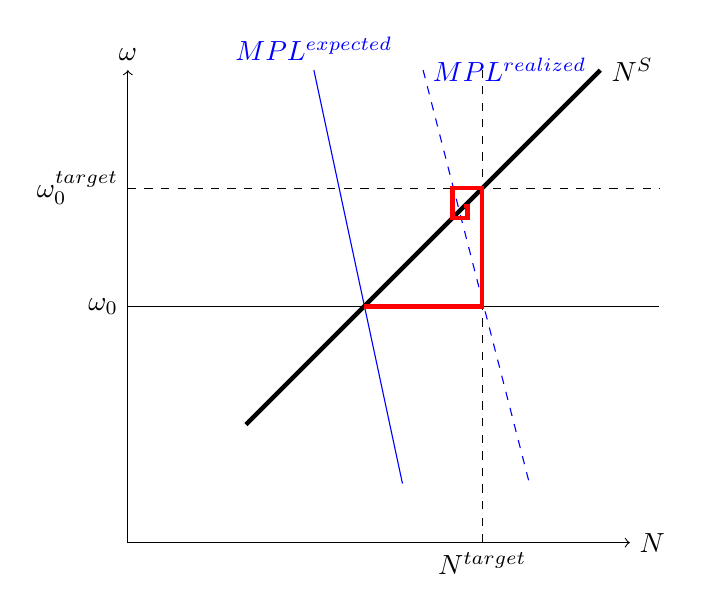
\begin{tikzpicture}[scale=.75]
% \draw[style=help lines,step=0.5cm] (-4,-4) grid (4,4)        [step=0.5cm]; %   (1,2) grid +(1,1);
% \node at (0,0){x};
 \draw[->] (-4,-4) -- (4.5,-4) node[right] {$N$};%
 \draw[] (-4,0)node[left] {$\omega_0$} -- (5,0);
\draw[dashed] (-4,2)node[left] {$\omega_0^{target}$} -- (5,2);
\draw[dashed] (2,-4)node[below] {$N^{target}$} -- (2,4);

 \draw[->] (-4,-4) -- (-4,4) node[above] {$\omega$};
%  \draw[->,red] (8,0.05) -- (8,3.2) -- (0.1,3.2)node[left] {$F(X^*)$};

\draw [ blue](-.85,4)node[above]{$MPL^{expected}$}-- (.65, -3); % 
\draw [ blue,dashed](1,4)node[right]{$MPL^{realized}$} -- (2.8, -3);
\draw [ ultra thick](-2,-2) -- (4, 4)node[right]{$N^S$}; 

\draw[ red, ultra thick](0,0) -- (2,0)  -- (2,2)--(1.5,2) -- (1.5,1.5)--(1.75, 1.5) --(1.75, 1.7)-- (1.7,1.7);%--(1.7, 1.6)--(1.7, 1.6) ;% node[right] {$X$};  CYCLING
    
 \end{tikzpicture}
    \caption {Labour market adjustment}
    \label{fig:cobweb}
\end{figure}

\begin{equation}
   \omega^{target}_{t}= c\sqrt(\frac{F_{t-1}n^{target}_{t-1}}{2 * density})
\end{equation}

Adjustment of  the labour market can be modelled as a cobweb process, as illustrated in the simplified cobweb Figure~\ref{fig:cobweb}. It is clear from the figure that the result of the market adjustment is that firms will be able to hire fewer than they target at a higher wage than they had enjoyed. 

\textbf{The slopes of the demand and supply curve would allow s to calculate the outcome. Both can be calculated  from the specified model. As a simple way of mimicking the market process we can simply calculate a partial adjustment, since we do not  expect a full equilibrium to be achieved in any period.}

For example
\begin{equation}
   \omega_{t}= 0.5 \omega_{t-1} +0.5 \omega^{target}_{t}
\end{equation}

The number of firms will also adjust as firms increase their capital stock and reduce their labour force in response to rising labour costs. At the same time, increasing employment will shift the marginal productivity curve outward.

\section{Where do we start?}
In each period we have the size of the existing workforce $N$ and the number of firms $F$ and $k_t$. \footnote{We also inherit the size of the existing firms. We can simplify by firms do not change their capital stocks as wages change. This would be incorrect but would do as a first approximation.}

\subsubsection{actual urban firms' employment} 
Aggregate labour supply is established by the process  above.  Available workers are divided among existing firms.   \begin{equation}
    n_t= \frac{N_t}{F_t} 
\end{equation}

From this, using the production function we can calculate the both output and  MPL

\textbf{urban firms' output}
\begin{equation}
    {y}_t=A_FN_t^\gamma k_t^{\alpha_F}n_t^{\beta_F}
\end{equation}

\textbf{urban firms'  marginal product of labour}
\begin{equation}MPL_{t} = \frac{\beta_{F}{y}_{t}}{n_t}\end{equation} 

This is used to calculate target employment.
% \item[(urban firms' capital)] (May not be needed)
% \[ K_{U,t}= \frac{\alpha}{\beta} \frac{n_{t-1}(\omega_{t-1}+\phi)}{r}\]
Firms observe their output, ${y}_t$ and find their $MPL_t$. They want to adjust labour so that the $MPL_t$ is equal to the wage. 




 \section{planning for the next period}

\subsubsection{urban firms' target employment for $t+1$} Firms examine their own output and marginal product of labour, all calculated with values determined in the previous period. 
Following the  optimality rule, for profit maximizing firms, MPL should equal the wage, $MPL_t= {\omega_t + \psi}$, however it doesn't because urban output includes the urban agglomeration effect. Effectively firms, are surprised. They take into account the effect due their own increase in labour. They don't take into account the overall effect on  productivity increase  through $N^\gamma$ due to every other firm increasing their labour force at the same time.
Firms thus compute a target value for $n_{t+1}$ based on the realized output  assuming the current wage. % They act like they are not changing the labour market by hiring more, however all firms hiring will actually affect the required wage, and they'll have to go back to revisit it. This uses simple equations to capture the dynamics of an itterative market process. 
\begin{equation} n^{target}_{t+1}= \frac{\beta_F {y}_{t}}{\omega_t + \psi} \end{equation}


%\subsubsection{number of firms}  Firm formation uses current variables to set number of firms for the next period. Decisions to enter or leave in the next period are based on current values. 
% \begin{equation}F_{t}=\frac{N_{t-1}}{n^{target}_{t-1}}\end{equation}
% . An increase in the number of firms adds to labour demand: 
% \begin{equation}
%     new\ firm\ demand = n^{target}_{t-1}(F_{t}-F_{t-1})
% \end{equation}


\textbf{urban firms' target capital for $t+1$} 
Firms also find their marginal product of capital, $MPK_t$ which should equality the cost of capital, $r$. 
\begin{equation}r= \frac{\alpha_{F}{y}_{t}}{k_{t}}\end{equation} 

Where $y$ is calculated using $n^{target}_{t+1}$
and adjust the capital stock so that the MPK$_t$ is equal to r. 

\begin{equation}k_{t+1}^{target}= \frac{\alpha_{F}{y}^{target}_{t}}{r}\end{equation} 
in period t should be based on planned output rather than the labour available in the period, so we begin with the marginal productivity of labour equation, 
which gives us 



\subsubsection{aggregate urban labour demand of existing firms $N_{F,t+1}^{target}$} 

\begin{equation}N_{F,t+1}^{target} = \frac{n^{target}_{t+1}}{n_{t}} N_t\end{equation}   
 % (This should be the same result as  multiplying $n^{target}_{t+1} \times F_{t} $.)

% Y is produced with the year's realized workforce.


{\color{red}}
\subsubsection{New entrant labour demand,  $n\Delta F$} Firms enter when $MPL > wage$, which with existing technology permits profit making. New firms would set the same target employment as existing firms. 
\begin{equation}n\Delta F =Z\frac{MPL_t-\omega_t -\psi}{\omega_t +\psi}F n^{target}_{t+1}\end{equation}
This makes sense because the number of entrants as a fraction of the existing number of entrants should be larger when the profit margin is larger. New firms would set the same target employment as existing firms and 

\subsubsection{Aggregate urban labour demand of existing firms $N_{Total,t+1}^{target}$} 
\[N_{Total,t+1}^{target}= N_{F,t+1}^{target}+n\Delta F\]

\subsubsection{Number of firm adjustment} 
\[F_{t+1}=\frac{N_{Total,t+1}^{target}}{n^{target}_{F,t+1}}\] 
This adjusts over time, keeping the firm labour force near the optimal level. 

\color{blue}
    \subsubsection{Wage adjustment for NEW workers} 
Firms want to increase output so they bid for new workers
\begin{equation}wage_t^{new}= (1-adj_\omega)\omega_{t-1} + adj_\omega MPL_{t-1}  +\psi\end{equation}
where $adj_\omega$ s the speed at which the wage (i.e., the wage the firm would offer for NEW workers) adjusts toward the Marginal product of labour for the firm]
\subsubsection{Wage adjustment for EXISTING workers }
Existing workers demand catch-up increases in wages

\begin{equation} wage_t^{existing}= (1-adj_{exist})*\omega_{t-2} + adj_{exist}* wage_{t-1}^{new}  +\psi 
\end{equation}
where $adj_{exist}$ is the speed at which the wage for existing workers adjusts toward the wage of new workers. This is a catch-up term.

Do we have to worry about workers switching firms? Would switchers get the full bid new workers get? I think the answer is yes. Say a fraction switched: It would have two effects. The catch-up ratio would be higher and the new workers hired would include workers from other firms. The target employment for the firm would not change, nor would the number of persons moving to the city in response to the higher wage. Only if the labour market were sticky would this have an effect.

A slow immigration response would have more effect.

This suggests that all workers could get the same wage.. Slow wage adjustment for existing workers would increase profitability and might make hiring more attractive, speeding the firm's labour adjustment.


\textbf{Labour force  adjustment factor $\nu$ (pronounced nu)} This is the fraction by which desired labour exceeds actual labour
\[\nu_t =\frac{N^{target}_{t+1}-N_{t}}{N_{t}}\]
or 
\[\nu_t =\frac{n^{target}_{t+1}-n_{t}}{n_{t}}\]



\subsubsection{Wage adjustment} 

\textbf{Wage calculation}
Firms make one decision faced with a market wage. They choose a target workforce. This is typical in \glspl{competitive market} where firms are price-takers. 


When \textbf{aggregate} firm labour demand exceeds N, wages rise at the city level

To get labour supply $N^s$ in terms of  $\omega$ we combine $N=f^2 *density$ and $f=2\omega/c$. 

So $\die{N^s}{omega}=4fden/c$ and \[\Delta \omega=  \frac{c}{4fden}\Delta N = \frac{c}{4fden}(N_{Total,t+1}^{target}-N_t)\]
This is the discrete wage adjustment that would attract the desired number of new workers, providing housing is available.\footnote{What happens is housing is not available? Maybe workers can't come to the city until the housing stock adjusts. Firms have labour shortages.  The wage stays high or may rise more. House prices will rise.} We can think of this as the wage demand of new workers.\footnote{What if only new workers get the new wage? This is interesting: firms will make excess profits. New firms will be attracted by excess profits but may not be able to get workers at the old wage!}

Should the adjustment occur in a single period?

It may be useful to put in an adjustment factor $adj \le 1$.
\[\omega_{t+1}=\omega_{t} + adj \Delta_t  \omega\]




% Common to think of the variations in local wages as variations around a mean, in this context - perfect labour market.
% We're using this number at the aggregate level, raise the market wage to a level that attracts that many. Divide available workers among the firms, then they want to raise the wage again. It's more transparent to do it at the aggregate level than at the firm level, but we still have the rising supply curve. A more detailed agent model could implement the hiring and wage adjustment mechanisms for firms directly, but the side effect of increased complication is it also can obscure the clarity of the rent results, our focus with this work. 



\section{Firm initial values}

\subsubsection{Firm $Y_{F,i}=A_FK_i^\alpha n_i^{\beta_F}$}
We use the familiar Cobb-Douglas production function \cite{chiangFundamentalMethodsMathematical2002} to set relationships among variables that are consistent with basic neoclassical production theory. 
\begin{description}

\item[initial urban wage premium] = $\omega_0 = (wage\_premium\_ratio) * \psi = p*\psi $

\item[initial labour force for urban firms] $n_0=n_R$.  Initially we will try values similar to the rural firm size and vary it  %*****%may have implica=tions later for the notation

\item[Initial wage premium] $\omega_0=p_0*\phi$

\item[Initial wage] = $\omega_0=\omega_t +\psi =(1+p_0)\psi)$
%The wage  is set as the marginal product of labour for initialization of the model. 

\item[labour cost for typical rural firm] $L_R = n_R*\psi$. This is expressed as a money quantity: e.g., 100 workers * \$40,000/worker.  

% \item[Initial labour cost for typical urban firm] ]  $L_U = n_R(\psi+\omega_0)$.

\item[output for typical rural firm]  
\[Y_R=\frac{n_R*\psi}{\beta_F}\]
This is a constant for any initial values. Derived from the marginal productivity condition. See item~\ref{item-paramlist-firm-level} in the orange  block. The numerical calculation is done  for a firm with 100 workers and a marginal product of labour of $\psi$. I get \$20 million for those values. 


\item[initial output for an urban firm] 
\[Y_0^U=N_0^\gamma Y^R\]  
Taking the marginal product with respect to $n$, we get a useful fact that will allow us to tie down $\gamma$
\[Y_{U,0}=\frac{n*(\psi+\omega)}{\beta_F}\]

\item[capital for typical rural firm] (Derived from the marginal productivity condition.)
\[K_R=  \frac{\alpha_R Y_R }{r}\]
This is also a constant.
 
\item[initial capital for an urban firm] (Derived from the marginal productivity condition.)
\[K_{U,0}=  \frac{\alpha Y_{U,0} }{r}\]
This is also a constant.

\item[scale factor A for typical  firm] 
\[A_F= \frac{Y_R}{K_R^{\alpha} {n\psi}^{\beta_F}}\]
We will assume that this is a constant used for both rural and urban production functions. (The explicit function is a bit  messy but the numeric value is easily computed because we have $L_r=n_R\psi$, and have calculated $Y_F$, and  $K_F$). The prefactor.

\end{description}
% \textbf{NOTE: With the initial values calculated in this section $\omega$ is consistent with $N_0$.as a result, population should not grow.}

\begin{quotation} \color{orange}
\section{Firm level production}   
(This is incorporated above.) We want the marginal product of labour in the rural economy at the firm level to be at least close to \$40,000.  We can create a generic rural firm and then consider an urban firm with agglomeration effects to get the parameters we need. 

Firm employment $L$ is small relative to  urban employment {N}. Assume it is 100 workers. 

Assume that the rural production function is 
\[ Y_{iF}^R=A_{F} K^{\alpha_F} L_F^{\beta_F} \]
where  $L_F=n*\psi$, $\alpha_F=0.18 $,  and $\beta_F=0.76$.notice that the MPL is the partial derivative with respect to $n$ and not L. 
\footnote{These values give us diminishing marginal product at the firm level. If we require product exhaustion we have factor shares of  0.8 and 0.2.The tricky point is that factor share are 
 $\frac{\alpha}{\alpha + \beta}$ and $\frac{\beta}{\alpha + \beta}$
(*If not there is surplus profit  which we will ignore.)}   
The marginal products pf labour and capital are 
\[MPL=n*\beta_F Y_F/L_F=\$40,000\] and\[\ MPK=\alpha_F Y_F/K_F =0.05\]
From the first, 

\[Y_F=\frac{n*\psi}{\beta_F}=\frac{100*\$40,000}{0.72}=\$5,555,556\]
This is firm revenue. From the MPK, 

\[K_F=  \frac{\alpha_F Y_F }{r}=\frac{0.18 *\$5.5555\ million}{0.05} =\$20\ million = 1.039568 \]

We now have the capital, labour and output for a model firm with a marginal product of labour  equal to the subsistence wage we have chosen. We can calculate the \textbf{scale factor} 

\begin{equation}  
A_F= \frac{Y_F}{K^{\alpha_F} L^{\beta_F}}=\frac{5,555,000}{20,000,000^{\alpha_F} 100^{\beta_F}} = 1.039568 \label{eqn-AR}\end{equation} 
So $A_F$ can be computed using equation~\ref{eqn-AR} for any set of coefficients and firm size. Expanding the expression,

% \begin{equation}  %   arithmetic error here
% A_F 
% =\frac{\frac{n*\psi}{\beta_F}}{\frac{\alpha_F  \left(\frac{n*\psi}{\beta_F} \right)}{r}  L^{\beta_F}} 
% =\frac{\frac{n*\psi}{\beta_F}}{\frac{\alpha_F \frac{n*\psi}{\beta_F} }{r}  L^{\beta_F}} 
% =\frac{r}{\alpha_F  L^{\beta_F} }
% =6.944444e-08???? \label{eqn-AR2}\end{equation} 

Furthermore, we can compute the output for a city of size N if it consists of $N/n$ firms of this type. With a population of 10,000, for example,  there would have to be  100 firms and an output of \$555,555,600. 

 \subsubsection{The urban level of production}
 \textbf{This section now redundant and has been commented out}
% We now consider that this firm operates in the city and enjoys  urban agglomeration benefits. The value of the  marginal product of labour must rise to $\psi+\omega$. We to know  the urban wage premium that is consistent with the subsistence wage. Papageorgiou \cite{papageorgiouOccupationalMatchingCities2022} found a 4.1\% premium. D'costa and Overman   show that working in London is associated with a 35.5\% higher wage than working in a rural area. The comparable figures are
% 10.6\% for big cities and 8.3\% for small cities and an elasticity of wages with respect to city size of 1.6\%.. Estimates of the premium are lower  when they control of individual characteristics.   

% If the $ scale\ coefficient=1.12$, $=\omega$ would be $1.12*\psi$, or $4,800$. 

% This supports an urban wage premium of $\omega\$8,000$.

% We need to have a population size or a number of firms with a firm size. Assume the population is 10,000 and firms still have 100 workers. (All firms will have the same marginal product of labour in a competitive labour market, so size should not matter.)

% \[Y^U=A^R N^\gamma K^\alpha L^\beta = N^\gamma Y^R\]
% where $N^\gamma$ represents the agglomeration effect. The marginal product of labour is 
% \[MPL^u=\$44,800=N^\gamma \beta Y^R/L=N^\gamma *\$40,000\]
% so $N^\gamma= 1.2$ and $\gamma = \frac{log(1.12)}{log(10,000)} =.012$. 


% This value is consistent with an empirical  value for  the agglomeration exponent of $\beta =  1.012$. The value is much lower than empirical estimates. Furthermore, if we consider the same firm structure and a population of one , the value falls, which suggests that agglomeration effects are not scale-independent, but instead increase with urban size. $\beta$ may itself be a function of $N$.

% % A second interesting possible implication of our calculation is that only part of the agglomeration effect appears in wages. Urban rents  are large, but agglomeration effects are much larger.
\end{quotation}



\footnote{Tørsløv et al \cite{torslovMissingProfitsNations2023} show that affiliates of foreign multinational firms are an order of magnitude more profitable than local firms in a number of low-tax countries. Leveraging this differential profitability, they estimate that 36\% of multinational profits are shifted to tax havens globally. US multinationals shift twice as much profit as other multinationals relative to the size of their foreign earnings.}


\textbf{appendix-05-agglomeration-model - REDUNDANT} %\renewcommand{\sfdefault}{phv}

\section{Initial values for  the agglomeration parameter}
A segment is now redundant and has been commented out

\vspace{5lines}

% {\Large  $Prefactor = 1506.712$ based on width=height=10 and density=100} and agglomeration\_coefficient= 1.2,
% We need to get the scales of the parameters and the population size roughly consistent.

% I assume the 10X10 grid is full. 

% \section{Computing the prefactor: details}
% We have set the subsistence\_wage to \$40,000.

% The urban wage premium is in the range of 13-20\%  Assume 20\% and we get \$8,000

% Under the neoclassical assumption  \$40,000 is the  marginal productivity of rural worker

% The urban production function is 
% \[Y=AN^\beta\]
% \[Y=prefactor*working\_population**scaling\_exponent\]

% where $working\_population = width*height*density$ 

% so 
% \[Y=prefactorA*(width*height*density)^{\beta}\]

% We have more conditions that this has to satisfy: The marginal product must be consistent with the urban wage and the distribution rule. The wage cannot add up to more than total output output. Workers cannot get 1.2Y/N, for example. With CRS they would get 0.8Y/N.    

% \subsection{approach one: from agglomeration surplus}
% \[urban\_wage= subsistence\_wage + wage\_share * agglomeration\_surlpus\]
% The \textbf{agglomeration surplus} is the excess relative to the CRS case when $\beta=1$:
% \[agglomeration\_surplus= A(N^{1.2} -N^1) \]
% The urban wage premium is then the share for each worker:
% \[\omega= wage\_share * \frac{agglomeration\_surlpus}{N}\]

% and this becomes
% \[\omega= wage\_share * A\left(\frac{N^{1.2}-N^1}{N}\right)=1 * A\left(N^{0.2}-1\right)\]

% To see what this looks like, consider a population of 10,000 when  wage\_share=1
% \[\omega= \$8,000 = A\left( 6.309-1 \right)\]

% {\Large So $A = 1506.712$ based on width=height=10 and density=100}  

% Smaller N makes A bigger

% % Say width=height=15 and density= 200:
% % \[\omega= \$8,000 = A\left(10000-1\right)\]

% \subsection{Approach 2: from Marginal product and subsistance wage}
% % We want the marginal product of labour in the rural economy at the firm level to be at least close to \$40,000.

% % Firm employment $L$ is small relative to  urban employment {N}.  We can create a generic rural firm and then consider an urban firm with agglomeration effects to get the parameters we need. 

% % Assume that the rural p[rooduction function is 
% % \[Y^R=A^R K^\alpha L^\beta\]
% % where $\alpha=0.2$  and $\beta=0.8$. The marginal products are 
% % \[MPL=\beta Y/L=\$40,000\] and\[\ MPK=\alpha Y/K =0.05\]
% % From the first, 

% % \[Y=\frac{L*\$40,000}{0.8}=\$5\ million\]

% % This is firm revenue. From the MPK, 

% % \[ \frac{0.2 \$5\ million}{0.05}=K =\$20\ million \]

% % We now have the capital, labour and output for a model firm with a marginal product of labour  equal to the subsistence wage we have chosen.

% % We now consider that this firm operates in the city and enjoys  urban agglomeration benefits.  If the scale coefficient=1.12$,$ $\omega$ would be as a first appr Say that the marginal product rises to \$48,000. This supports an urban wage premium of $\omega\$8,000$.

% % We need to have a population size or a number of firms with a firm size. Assume the population is 10,000 and firms have 100 workers. All firms will have the same marginal product of labour in a competitive labour market, so size should not matter. 

% % \[Y^U=A^R N^\gamma K^\alpha L^\beta = N^\gamma Y^R\]
% % with a marginal product of 
% % \[MPL^u=\$48,000=N^\gamma \beta Y^R/L=N^\gamma *\$40,000\]
% % so $N^\gamma=1.2$ and $\gamma = .019$. 


% This value is consistent with an empirical  value for $\beta$   1.02. The value is lower than empirical estimates. Furthermore, if we consider the same firm structure and a population of one million the value falls, which suggests that agglomeration effects are not scale-independent, but instead increase with urban size. $\beta$ may itself be a function of $N$.

% A second interesting possible implication of our calculation is that only part of the agglomeration effect appears in wages. Urban rents  are large, but agglomeration effects are much larger.


 

% %\[subsistance_wage= MPL(\beta=.= \]
 % bbbb{appendix-05-agglomeration model}



\begin{enumerate}
\item To start with a population of around 10,000, we begin with width = 10, height = 10 and \textbf{density} per unit of 100. 

\item If we arbitrarily assume an initial wage premium around 20\%, and wish to start near equilibrium, % bettencourt assumed aggomeration exponent is indepent)
we can select transportation costs. A transportation cost of 0.1  would give a distance of $\omega/.01$, which is huge. Could this be 1/10 of the starting wage premium $\omega_0$? It would then be \$800 per year, per unit distance and would give us height and width of 10. 
% (divide into omega) - we want to start close to equilibirum. omega/cost = width
\item We should have a wage premium of about \$8000 to be consistent with the subsistance wage. % since we are assuming the wage premium of around 20%. Total wage has to be subsistence wage + wage premium, think of an average rural subistance wage seems like 45K .. 

\item Your proposed prefactor was 0.2,  251. It should be very large, based on the above numbers and the consistency constraints. I get 1507 in appendix-05-agglomeration model

\item Teminology: Y=prefactor*N**scaling\_exponent

\end{enumerate}

\subsection{Workers share}
The worker's of the surplus, $lambda$ It might be 0.8. It is used in...

NOTE: 0.8 is the value of beta in a Cobb-Douglas, corresponding to the wage-share in production. It is the value used in Lobo et al


